\documentclass[11pt,a4paper]{report}
\usepackage[latin1]{inputenc}
\usepackage{amsmath}
\usepackage{amsfonts}
\usepackage{amssymb}
\usepackage{graphicx}
\usepackage{url}
\usepackage[left=2.50cm, right=2.00cm, top=2.00cm, bottom=2.00cm]{geometry}
\author{He Xiao (netid: hexiao2)}


\usepackage{sidecap}
\usepackage{caption}
\usepackage{color}
\definecolor{name}{rgb}{0.5,0.5,0.5}
\usepackage{listings}

\lstset{ %
  backgroundcolor=\color{white},   % choose the background color; you must add \usepackage{color} or \usepackage{xcolor}
  basicstyle=\footnotesize,        % the size of the fonts that are used for the code
  breakatwhitespace=false,         % sets if automatic breaks should only happen at whitespace
  breaklines=true,                 % sets automatic line breaking
%  captionpos=b,                    % sets the caption-position to bottom
  commentstyle=\color{green},    % comment style
  morecomment=[s][\color{green}]{/*}{*/},
  deletekeywords={...},            % if you want to delete keywords from the given language
  escapeinside={\%*}{*)},          % if you want to add LaTeX within your code
  extendedchars=true,              % lets you use non-ASCII characters; for 8-bits encodings only, does not work with UTF-8
  frame=single,                    % adds a frame around the code
  keepspaces=true,                 % keeps spaces in text, useful for keeping indentation of code (possibly needs columns=flexible)
  keywordstyle=\color{blue},       % keyword style
  language=[Sharp]C,                 % the language of the code
  morekeywords={},            % if you want to add more keywords to the set
  numbers=left,                    % where to put the line-numbers; possible values are (none, left, right)
  numbersep=5pt,                   % how far the line-numbers are from the code
  numberstyle=\footnotesize, % the style that is used for the line-numbers
  rulecolor=\color{black},         % if not set, the frame-color may be changed on line-breaks within not-black text (e.g. comments (green here))
  showspaces=false,                % show spaces everywhere adding particular underscores; it overrides 'showstringspaces'
  showstringspaces=false,          % underline spaces within strings only
  showtabs=false,                  % show tabs within strings adding particular underscores
  stepnumber=1,                    % the step between two line-numbers. If it's 1, each line will be numbered
  stringstyle=\color{red},     % string literal style
  tabsize=2,                       % sets default tabsize to 2 spaces
  framexbottommargin=4pt,
  belowcaptionskip=-2em,
}


\DeclareCaptionFont{white}{ \color{white} }
\DeclareCaptionFormat{listing}{
\begin{flushleft}
   \colorbox{cyan}{
    \parbox{\textwidth}{\hspace{0pt}#1#2#3} 
  }
\end{flushleft}
}
\captionsetup[lstlisting]{ format=listing, labelfont=white, textfont=white,justification=justified, singlelinecheck=false, margin=-10pt, font={bf,footnotesize} }

\title{CS477 Course Project Report}
\begin{document}

\maketitle

\section*{Abstract}
Design by contract is a popular design pattern that has been widely used to increase the reliability of software systems. This kind of programming paradigm requires the programmers to provide formal, precise and verifiable interface specifications for software components\cite{wiki:dbc}. Dafny\cite{dafny1} is such a language that enables programmers to provide contracts for various program constructs and the tool with the same name can verify functional correctness of programs written in this language. The author of this report used dafny to develop and verify the correctness of operations on a singly-linkedlist, including insert, delete, get, indexOf, update. All the operations were implemented in iterative fashion (use loops instead of recursion). For most of the operations, the author also came up with a recursive version which required much fewer efforts to develop and can be proved by Dafny much faster compared to the iterative counterpart. The author also made a small contribution to the Dafny project by reporting a small bug in dafny script (see http://dafny.codeplex.com/workitem/90).
\section*{Introduction}
Dafny uses the concept of ghost variables to facilitate the proof of operations on complex data structures. The ghost variables are only for verification purposes and will be removed before generating the executable code.\\

The class invariant is built manually via a predicate function Valid(), which will be checked before and after each operation. The assertion of class invariant establishes the isomorphism between the 'real' data structure (under verification) and the ghost data structure which is only for verification purpose. If the isomorphism is preserved after the operation, furthermore the updated ghost structure and the old ghost structure before the operation have certain relation, then we can expect the same relation holds for the updated 'real' data structure and the old 'real' structure before the operation.\\

For example, the ghost field 'footprint' of a node X is a set that contains exactly all the nodes that are reachable from the node X via repeatedly applying the 'next' relation. If after some operation a new node Y is included in the footprint of X, and the corresponding predicate related to 'footprint' still holds, then there must be a path from X to Y.\\

Later in the report, I will explain how to use Dafny to verify the operations on a singly-linked list in the implementation section; the performance of verifying the properties will be listed in the evaluation section; and I will also share the experience of using the Dafny tool in the Learning Points section.
\section*{Implementation}
To prove the same method contract expressed as pre/post-condition, it is easier to use recursive approach compared to iterative approach (which involves loops and loop invariant). It is natural for humans to think about questions in top-down manner and solve them via divide and conquer; as a result, it is easier to come up with the recursive functions that persuade Dafny that the method contracts have been satisfied by the implementation. However, the project is required to develop Dafny code that use loop invariant, therefore, only the iterative approach will be discussed here.

\bigskip
In this section, the implementation and proof of delete method (which is the most complex one) will be exemplified. The other methods were implemented and proved in a similar way and will be skipped here.\\

The implementation of method delete(index:int) is divided into two classes: INode and INodes respectively. This is for the convenience of handling the situation where the last node is deleted from the list. There is a dummy node in the INodes that never gets deleted, storing no list data but pointing to the first real node in the list.

\subsection*{Fields and ghost fields of class INode}
\begin{lstlisting}
ghost var tailContents: seq<Data>;
ghost var spine: seq<INode>;
ghost var footprint: set<INode>;

var data: Data;
var next: INode;
\end{lstlisting}

There are two fields in a linked-list node: data and next, where the data can be of any type, and next is of type INode which denotes the next node referenced by the current node.\\

The three ghost variables, namely tailContents, spine and footprint, represent the data sequence starting from the next node, the whole list in sequence form, and the reachable nodes from the current node, respectively.

\subsection*{class invariant for INode}
\begin{lstlisting}
predicate good()
reads this, footprint;
{
    this in footprint 
	&& (next != null ==> (next in footprint 
	&& this !in next.footprint 
	&& footprint == {this} + next.footprint
	&& spine == [this] + next.spine
	&& tailContents == [next.data] + next.tailContents
	))
	&& (next ==null ==> tailContents == [] && footprint == {this}
				&& spine == [this])
}

predicate Valid()
reads this, footprint;
{
good()  
&& (next != null ==> next.Valid())
}
\end{lstlisting}  

The predicate $Valid()$ in the above code defines the class invariant of a linked-list node. It describes the structural property of the linked list, for both the singleton list and list with more than one nodes. This property is held since the object of the INode is created by the constructor, and will be maintained by all the operations performed on the object.

\begin{figure}[htbp]
\centering
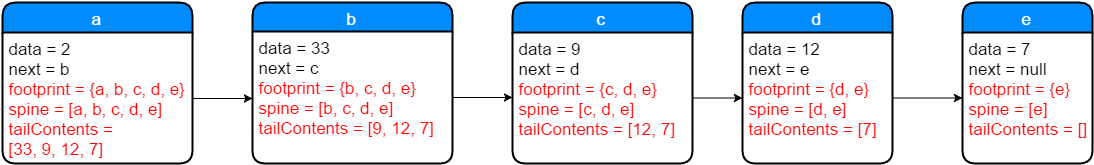
\includegraphics[width=0.81\textwidth]{./Diagrams/ValidLinkedList}
\caption{The graph notation of a valid linked-list}
\label{fig:ValidLinkedList}
\end{figure}

\subsection*{A heavily used lemma}

\begin{lstlisting}
predicate ValidLemma()
requires Valid();
reads this, footprint;
ensures ValidLemma();
ensures (forall nd :: nd in spine ==> nd in footprint);
ensures |tailContents| == |footprint|-1 == |spine|-1;
ensures forall nd :: nd in spine ==> nd != null && nd.Valid();
ensures forall nd :: nd in footprint ==> nd != null && nd.Valid();
{
if next == null then (spine == [this])
else (
spine == [this] + next.spine 
&& next.ValidLemma())
}

\end{lstlisting}

The ValidLemma() summarizes some valid consequence of the Valid() property which helps the procedure of proving complex properties. 

\begin{lstlisting}
	method delete(pos:int) returns (delNd:INode)
	requires Valid();
	requires 0 < pos <= |tailContents|;
	
	modifies footprint;
	
	ensures Valid();
	ensures [data] + tailContents == old(([data] + tailContents)[0..pos] + ([data] + tailContents)[pos+1..] );
	ensures footprint == old(footprint) - {delNd};
	
	{
	var curNd := this;
	var curIndex := 0;
	
	assert ValidLemma();
	assert ndValid2ListValidLemma();
	assert validSeqContentsLemma();
	assert validSeqTCLemma(spine);
	
	while (curIndex < pos-1)
	invariant 0 <= curIndex < pos;
	invariant curNd != null && curNd.Valid();
	invariant validSeqCond(spine);
	invariant |curNd.tailContents| + curIndex == |tailContents|;
	invariant curNd.next != null;
	invariant curNd == spine[curIndex];
	
	invariant  spine[curIndex].data == ([data] + tailContents)[curIndex];
	
	invariant curNd.next == spine[curIndex+1];
	invariant curNd.next.next != null ==> curNd.next.next == spine[curIndex+2];
	
	modifies {};
	{
	curNd := curNd.next;
	curIndex := curIndex + 1;
	}
	
	delNd := curNd.next;
	
	delNext(curNd, delNd, pos);
	
	
	if(1 < pos <= |tailContents|) {
	ghost var oldContents := old([data] + tailContents); 
	ghost var newSpine := spine[0..pos-1];
	
	assert delNd != null;
	
	updateSeq4Del(newSpine, delNd, pos, curNd, oldContents, this);
	
	} else {}
	
	}
\end{lstlisting}

To present the structure of proof more clearly, the operation of delete is divided into three parts: the first part contains a loop that iterating the list and stops at the node whose next one is the node that is going to be deleted. Then the deletion is achieved by the second part, which is an invocation of the method delNext(curNd:INode, delNd:INode, pos:int); Finally, the ghost variables are updated in the ghost method 'updateSeq4Del'; This layout gives a clearer structure and also enables me to specify accurate frame conditions neatly for each sub-operation.

\bigskip

The code to prove the delete(index:int) operation used several predicates, some of them specify the properties held by different portions of the list at certain program points; others specify the properties held by the whole list, but with different strength, which reflect the properties held by the whole list at different phases. Certain predicates are not directly clear but can be deduced by providing proper lemmas. In the next section, several predicates used in the code will be exemplified.

\subsection*{Some Predicates}
\begin{lstlisting}[caption=valid sequence predicate]
predicate validSeqCond(mySeq: seq<INode>)
reads mySeq, (set nd | nd in mySeq);
{
listCond(mySeq) 
&& (mySeq != [] ==> mySeq[|mySeq|-1].next == null
&& mySeq[|mySeq|-1].footprint == {mySeq[|mySeq|-1]}
&& mySeq[|mySeq|-1].tailContents == []
&& mySeq[|mySeq|-1].spine == [mySeq[|mySeq|-1]])
}
\end{lstlisting}

The predicate of valid sequence defines the property of a valid sequence which is isomorphic to a linked-list. So, given a valid linked-list node, its ghost field 'spine' must satisfy the validSeqCond property. And vice versa, given a valid sequence, the first node of the sequence must be valid and its spine field must be equal to the whole sequence.

\bigskip
When some node in the list is updated, it will break the properties of all the nodes from which the changed node can be reached, while the next node linked by the changed node will not be affected. For example, the 'i'th node in a list is updated, then it will immediately invalidate all the nodes with indices less than or equal to i, however, all the nodes with indices that are large than i will not be affected.

\bigskip
Even though the stronger property 'validSeqCond' may not hold after a change in the member node, some weaker properties of the list may still hold, like the property 'listInv'\\

\begin{lstlisting}[caption=list invariant property]
predicate listInv(mySeq: seq<INode>)
reads mySeq, (set nd | nd in mySeq);
{
null !in mySeq && (forall nd :: nd in mySeq ==> nd in nd.footprint) &&
(forall i :: 0 <= i < |mySeq|-1 ==> mySeq[i].next == mySeq[i+1])
&& (forall i, j :: 0 <= i < j < |mySeq| ==> mySeq[i] !in mySeq[j].footprint)
}
\end{lstlisting}

\bigskip
In the case where the $i$th node is deleted, then the No.$i-1$ node's next field will be set to point to No.$i+1$ (if there is any) (we require the first node should not be deleted in INode class). Because nothing in the subsequence of $spine[0..i]$, say $s_1$, is changed except the next field of the last element in $s_1$, so the following $listCond$ property is held on the sequence $s_1$. 

\begin{lstlisting}
predicate listCond(mySeq: seq<INode>)
reads mySeq, (set nd | nd in mySeq);
{
null !in mySeq && (forall nd :: nd in mySeq ==> nd in nd.footprint) &&
(forall i :: 0 <= i < |mySeq|-1 ==> mySeq[i].next == mySeq[i+1]
&& mySeq[i].footprint == {mySeq[i]} + mySeq[i+1].footprint
&& mySeq[i].tailContents == [mySeq[i+1].data] + mySeq[i+1].tailContents
&& mySeq[i].spine == [mySeq[i]] + mySeq[i+1].spine)
&& (forall i, j :: 0 <= i < j < |mySeq| ==> mySeq[i] !in mySeq[j].footprint)
}
\end{lstlisting}

\bigskip

Another segment of the spine field, say $s_2 = spine[i+1..]$, is the same as before, so it is still a valid sequence which satisfies $validSeqCond$ property.\\

Therefore, to make the all the nodes in the list become valid again, we only need to update the ghost fields in sequence $s_1$ so that the ghost fields reflect the real data structures. In the sequence $s_1$, we also observes that $s_1[i+1]$ is valid if $i+1$ is a valid index of the sequence $s_1$.

\bigskip

So at this moment, we actually have already found the loop invariant which enables us to prove the Valid() property after updating the nodes in the sequence $s_1$. We did the proof inside the following separate ghost method called $updateSeq4Del$\\

\begin{lstlisting}
ghost method updateSeq4Del(newSpine: seq<INode>, delNd:INode, pos: int, nxtNd:INode, oldContents:seq<Data>, thisNd:INode)
\end{lstlisting}


The above code snippet is inside a separate method which is dedicated for updating the ghost variables, and when it is invoked, the caller will send $old([data] + tailContents)$ as argument for the parameter $oldContents$, which reflects the content of the list before performing the delete operation.\\


To perform the iterative updates, we need to traverse the nodes in the sequence from right to left; and in the loop body, we need to update the footprint, tailContents and spine field of the node at that iteration (i.e. node with index $i$) so that the node $s_1[i]$ visited at that iteration becomes valid again. Then we decrement the index i so that 
the loop invariant holds again: $s_1[0..i]$ and  $s_1[i+1..]$ satisfies the  $listCond$ property, and $s_1[i+1]$ is valid.\\

At the end, when we exit the loop, index i becomes -1 and therefore the first node $s_1[0]$ in this sequence, which is the node upon which we performed the delete operation, is valid.

\bigskip

However, we should not stop here; it is easy to provide an implementation that makes the current node valid after the operation, we can in fact delete everything except the first node and still makes the node valid; but that's not desirable.
Therefore, we need to ensure another post condition: $[data] + tailContents == old(([data] + tailContents)[0..pos] + ([data] + tailContents)[pos+1..] );$ through which we can guarantee that we only delete the data at the specified position.\\

We proved that post condition by adding the following loop invariant into the loop's annotation block:\\

$invariant -1 <= curIndex < pos - 2 ==>  [newSpine[curIndex+1].data] + newSpine[curIndex+1].tailContents == oldContents[curIndex+1..pos] + oldContents[pos+1..];$\\

$	invariant thisNd == newSpine[0];$\\

When we exit the loop, curIndex becomes -1 and we can get the desired post condition about list contents successfully.

\subsection*{Implementation Style}
During the implementation, besides the traditional method invocation and while loops, I also tried something similar to the \emph{Basic Path} approach for generating the verification condition. Basically, I identified different parts of the method which are separated by pre/post conditions and loop invariants, and implemented the following methods/predicates:\\

\begin{itemize}
\item LI: predicate for expressing loop invariant.
\item pre2LI: which is a method that verifies executing the initialization code at the state which satisfies the pre-condition will result in a state which satisfies the loop invariant.

\item LIGuardExecBody2LI: Executing the loop body in a state which satisfies the loop invariant and loop guard will result in a state that still satisfies the loop invariant.

\item LIAndNegGuard2Post: it is in fact a lemma that checks the fact that loop invariant together with the negation of the loop guard will imply the post condition.
\end{itemize}

\section*{Evaluation}
The Dafny software used in this project was built from source, and the dafny code that I developed was tested both on windows and ubuntu system.\\

The most reliable way to reproduce the results is to verify the programs on ubuntu system, because I noticed that some complex program (specifically, the one related to delete operation) can only be proved efficiently on Ubuntu platform.

\bigskip

Most operations/lemmas can be verified in several seconds, some more complex may need longer but usually not exceeding half a minute.\\

Comparing with recursive approach, iterative approach is more complex and potentially slower for verification. The rationale of implementing the code in iterative fashion is that the iterative approach is more efficient in execution; and deliver a verified version of the iterative implementation is quite attractive because we only need to verify the code once and then we can trustfully use it since then.
\section*{Learning Points}
\subsection*{LI is very important}
It is vital to come up with the right LI, so that the loop can be proved which is necessary for proving the total correctness of program. It is important to carefully analyse the relation that remain unchanged during the iterations. The stronger property may not hold after some update, but possibly the weaker version already suffices. Sometimes it is hard to find the invariant for the whole structure, then it may be helpful to divide the elements into different segments/partitions according to their satisfying properties. After we made some separate conclusion on the new abstraction level, we may observe how the properties change between different statements of the loop body; if the conclusion hold at the beginning of the iteration and after executing one iteration, it holds again, then we find a loop invariant. 

\subsection*{Dafny is well documented language}
There is a detailed online tutorial for Dafny, where every program construct and language feature have been explained and the usage of operations are exemplified well. I have learned deeply how to write Dafny programs with different built-in types and lemmas to prove functional correctness. It is vital to provide the most accurate frame conditions for functions (reads clause) and methods (modifies clause) so that the proof can be performed smoothly. It is also very important to provide proper lemmas to facilitate/accelerate proof process. 

\subsection*{Dafny tool is NOT documented}
In contrast to the language, the Dafny tool does not have documented API and it is difficult to find the available command-line options. I found the full list of command-line options by investigating the source code of Dafny.


\subsection*{Dafny tool has performance bug and does not scale up}
The following observations are summarized from my experiments:\\

\begin{itemize}
\item  Unused lemmas may degrade the performance of verification dramatically even if they can be efficiently verified independently. A hypothesis for this phenomenon is adding the junctions(unused lemmas) may decrease the chance of targeting and selecting the truly needed lemma. 

\item Moving the lemmas from class level to module level seems increasing the efficiency.

\item Adding an assertion (through pre/post or assert statement in the method body) at method A may have significant influence on the time used to prove some other method B. This is quite annoying and unpredictable. 

\item Even if two methods can be efficiently verified separately, merging them into one big file will slow down the proof dramatically. In one experiment, two files can be verified in 24 seconds and 33 seconds respectively, but merging them into one big file took over half an hour to verify. The overhead really goes fast.

\end{itemize}

\subsection*{Some comparison of editor of Dafny Code}
In the early stage of the project, I tried to use the Visual Studio as a platform and had the dafny installed as a plug-in; however, that is not very good choice for developing large piece of dafny code, because there are too many false positives and Visual Studio does not provide clear answer quickly.\\

After some time of using plain text editor, I found emacs with boogie-friends plug-in is very powerful and suitable for the development of dafny code; not only because it provides the syntax highlighting, but also because it integrates the dafny compiler so that I can easily compile my code via pressing key combination and see the output in the same window after I am satisfied with the code.\\


 
\section*{Acknowledgement}
Thanks Edgar and Madhu for explaining the project aim and giving instructions for how to find relevant resources.

\bibliographystyle{plain}
\bibliography{ref}

\end{document}